\documentclass[10pt,twocolumn,letterpaper]{article}

\usepackage{cvpr}
\usepackage{times}
\usepackage{epsfig}
\usepackage{graphicx}
\usepackage{amsmath}
\usepackage{amssymb}

% Include other packages here, before hyperref.

% If you comment hyperref and then uncomment it, you should delete
% egpaper.aux before re-running latex.  (Or just hit 'q' on the first latex
% run, let it finish, and you should be clear).
\usepackage[breaklinks=true,bookmarks=false]{hyperref}

\cvprfinalcopy % *** Uncomment this line for the final submission

\def\cvprPaperID{****} % *** Enter the CVPR Paper ID here
\def\httilde{\mbox{\tt\raisebox{-.5ex}{\symbol{126}}}}

% Pages are numbered in submission mode, and unnumbered in camera-ready
%\ifcvprfinal\pagestyle{empty}\fi
\begin{document}

%%%%%%%%% TITLE
\title{Convolutional Neural Nets for the MNIST Digit Dataset}

\author{Reymundo A. Gutierrez\\
Massachusetts Institute of Technology\\
{\tt\small ragtz@mit.edu}\\
% For a paper whose authors are all at the same institution,
% omit the following lines up until the closing ``}''.
% Additional authors and addresses can be added with ``\and'',
% just like the second author.
% To save space, use either the email address or home page, not both
\and
Juli\'{a}n A. Gonz\'{a}lez\\
Massachusetts Institute of Technology\\
{\tt\small jugonz97@mit.edu}
}

\maketitle
%\thispagestyle{empty}

%%%%%%%%% ABSTRACT
\begin{abstract}
   Should we put an abstract here?
\end{abstract}

%%%%%%%%% BODY TEXT
\section{Introduction}

Object recognition, the problem of mapping an image to a class label, is one of the core
problems in computer vision.
A related fundamental problem is object detection, also commonly referred to as object recognition.
(To avoid ambiguity, here we will define object detection as detecting and localizing objects and
performing object recognition).
The applications of object recognition and detection are endless, from simple visual search of
images to high-level scene understanding. It is by no means a solved problem.
This paper provides a survey of the current landscape of approaches toward the problem,
laying a conceptual foundation for the design and implementation of a convolutional neural net for
digit recognition.

Modern approaches towards object recognition differ significantly but tend to depend on
properties of images (features) that are not disturbed during transformations.
As an example, \cite{LoweObjSIFT} informed the computer vision community about the importance of
local scale-invariant features on images.
These lower-level features are still useful in innovative systems, but because of their
locality are hard to utilize alone.
Relationships between features can be leveraged to determine higher-level structure of
objects with careful estimation \cite{PartModels}.
Higher-level structure can be thought of as a hierarchy, which allows for composition of features \cite{HintonDBN}.
With such a hierarchy it is possible to look for translation-invariant features \cite{CDBN}.
This demonstrates that the difficulty of object recognition often lies in determining
appropriate representations of image data.

Convolutional neural nets recognize this difficulty and tackle it by iteratively tuning randomly
initialized filters (that act on all locations of an image) to produce a well-known output using
the back-propagation algorithm. These neural nets are convolutional because the convolution operator
is used to effectively share filters across an entire image. While time-consuming to train, CNN's
can provide world-class performance on a large and diverse dataset \cite{ImageNet}.
To gain a deeper understanding of the challenges of implementing an object recognition system,
we designed and implemented a convolutional neural net and tested it on the popular MNIST
digit dataset \cite{MNIST}.
To examine the effect of the number of layers in convolutional neural networks,
we trained two versions of our net with different depths on the MNIST training data
and compare their performance here.

The rest of this paper is organized as follows.
Section 2 provides an overview of several modern approaches to object recognition
roughly in chronological order, to make it easier to see how strikingly different
solutions to the same problem have evolved.
Section 3 shows how we use ideas from these approaches to design
a convolutional neural network for recognizing hand-written digit data.
Section 4 describes our implementation of a CNN.
Section 5 highlights the performance of our CNN in different conditions and with different depths.
Section 6 concludes with a discussion of the implications of our results, and ideas for
further work.

%------------------------------------------------------------------------
\section{Review of Methods}
\subsection{Scale-Invariant Feature Transform}

One way to begin to perform object detection / recognition is to identify discriminating
features of the object (i.e. features that can be mapped to a specific object or class of
objects with high probability). It is also necessary for robustness that these features
possess a certain degree of invariance to changes in translation, rotation, scale, and
illumination. The scale-invariant feature transform (SIFT) algorithm focuses on detecting
such features \cite{LoweObjSIFT}.

SIFT features are generated by first locating points that have translational, rotational,
and scale invariance by finding the maxima and minima of a difference of Gaussians
applied to an image pyramid. Each point is then assigned a canonical orientation
determined by the peak in a histogram of local image gradient orientations. To add
robustness to local geometric distortion, each point can be represented by a set of
images at different orientations and its encapsulated gradients at each orientation,
with intermediate gradients being determined through interpolation and blurred for
added translational invariance.

Object detection through SIFT features is fairly robust and can even function under
occlusion when many features are used to represent an object.

%-------------------------------------------------------------------------
\subsection{Part Based Models}

\cite{PartModels} models objects as collections of smaller parts.
In a part-based model, object parts are connected to each other via springs that
allow constrained deformation. This allows the construction of part-specific filters.
In addition, a root filter that is tuned for the entire object operates at half
the spatial resolution as the part filters, allowing for multi-spatial recognition.
Object detection in this scheme uses the best set of part filter responses given a
location for the root filter.

Because the training data used only contains bounding boxes for objects,
part locations must be learned. Training is done using a specialized latent support
vector machine that identifies part locations. Effort is also taken to locate a
number of difficult negative examples for specialized training.

Part-based models can be computed efficiently: dynamic programming algorithms
can be used to calculate part locations and the system in \cite{PartModels} can be trained
and run on a real dataset in less than 8 hours.
This system however has not aged well: the canonical implementation's average precision
scores on the PASCAL VOC 2007 \cite{PascalVOC} test have been eclipsed in recent years
by convolutional neural nets.

%-------------------------------------------------------------------------
\subsection{Deep Belief Networks}

While the methods discussed previously explicitly describe the features to be used
by the representation, deep belief nets (DBN) allow for the discovery of such features
from a training set \cite{HintonDBN} \cite{CDBN}.
DBNs, like parts-based models, also look at the relationship between features of an object,
but do not constrain the type of relation.
Instead, DBNs build a hierarchical representation of the object with each level of the hierarchy
representing more abstract features.

The basic component of a DBN is the restricted Boltzmann machine (RBM).
An RBM is a bipartite, undirected graphical model that can learn a probability distribution
over its inputs and whose edges are represented by a weight matrix.
Being bipartite, the RBM forms two layers; the layer associated with the input is known
as the visible layer and the other as the hidden layer.
Following the probabilistic semantics laid out in \cite{CDBN}, the weight parameters of the RBM
are optimized by performing gradient-based contrastive divergence, which utilizes a
Gibbs sampling step on the conditional probability of the hidden and visible units given
the visible and hidden units respectively.
These conditional probabilities are known as the output function, which often take the form of a sigmoid.
The DBN is then constructed by stacking RBMs into several layers.
The whole network is trained by greedily training each layer in succession up the hierarchy,
freezing the parameters of each previous layer.
To produce class labels, either the labels are included as input or a classification algorithm
can be trained on the higher level features.

DBNs are successful on classification tasks in certain domains, such as the MNIST digit recognition
task \cite{HintonDBN}. Unfortunately, they are difficult to scale to realistically sized images
due to the representational redundancy needed to compensate for their loss of image
two dimensional structure. This loss also makes translational invariance difficult to achieve.

%-------------------------------------------------------------------------
\subsection{Convolutional Neural Networks}

We can construct a different way to use a hierarchical representation of an image for classification
by performing convolutions at different scales of images with sets of filters.
Convolutional Neural Nets (CNNs) use a combination of convolutional layers, which perform convolution
of an image with a set of filters, and pooling layers, which reduce the dimensionality of the output
of convolutional layers, to create this representation. Convolutional layers serve to share the filter weights
across the image and thus reduce the number of parameters that must be trained, while also providing
a certain degree of traslational equivariance.
Pooling layers reduce dimensionality by taking the maximum value (max-pooling) or mean value
(mean-pooling) of a region of convolutional outputs.
This reduction of dimensionality is important because it helps reduce the number of parameters that
must be trained in the network, thus speeding up learning.

Modifications to this architecture \cite{CDBN} have produced some of the most performant
systems to date.
By overlapping hidden layer blocks during max-pooling, \cite{ImageNet} increases performance.
The approach outlined in \cite{Verydeep} gains significant accuracy by constructing a net with
a large number of convolution and pooling layers (using very small filters).

In order to counter the extra complexity introduced by these changes,
\cite{ImageNet} and \cite{Verydeep} replace the standard sigmoid nonlinear output function with the
Rectified Linear Unit (ReLU) function $f(x) = max(0, x)$ for quicker training.
Additionally, both use multiple GPUs for significant speedup in matrix operations
and easy parallelism.
Nevertheless, these CNNs take a very long time to train: the net in \cite{Verydeep}
takes 2-3 weeks to train using four GPUs.

%-------------------------------------------------------------------------
\subsection{Convolutional Deep Belief Networks}

The idea of using convolution can also be applied to Deep Belief nets.
To address the scalability and translational invariance issues inherent in DBNs,
Lee \etal introduce the convolutional deep belief network (CDBN),
which augments DBNs with convolutional restricted Boltzmann machines (CRBMs)
and probabilistic max-pooling layers between CRBMs \cite{CDBN}.
Like RBMs, CRBMs consist of a visible layer and hidden layer, but the hidden
layer here is partitioned into $K$ square blocks, each associated with a filter
whose weights are shared amongst the units in a block.
The relation between the visible units and the corresponding hidden units in each
block is defined by a convolution of the weight matrix and the image.

To alleviate the scaling issue, a probabilistic max-pooling layer is added above the CRBM,
forming a max-pooling CRBM.
These pooling layers contain $K$ blocks, with each block mapping to the corresponding hidden
layer block below it as follows: the hidden layer block is partitioned into square blocks with the
corresponding pooling unit for each block being set to 1 if and only if a unit in its hidden layer
block is 1, of which only one can be non-zero.
The CDBN is constructed by stacking max-pooling CRBMs, which are trained similarly to RBMs.

The training of CDBNs is accomplished using the same greedy approach as in DBNs.
Once the parameters have been learned, the CDBNs representation of an image can be computed
by sampling from the joint distribution over all the hidden layers given the input image.
The classification of images can be produced by training a classification algorithm
on the higher level features.

Because CDBNs construct a hierarchical representation of their input that is robust
to appearance, scale, and occlusion variation, they are are able to deliver
state-of-the-art performance.
They are not without shortcomings: in particular, they suffer from over-fitting due
to over-representation of their input data.
There are several solutions to this problem. In dropout, the output of a hidden layer
unit is set to 0 with probability $\frac{1}{2}$; this unfortunately significantly increases training
time (which can already take weeks). Another common solution, data augmentation,
is to insert altered forms of the input images into the dataset
(a good description of this idea is provided in \cite{Verydeep}).

%-------------------------------------------------------------------------
\section{CNN Design}

Utilizing some of the ideas outlined for object recognition in section 2,
here we will outline the design of a convolutional neural network to recognize
handwritten digits from the MNIST database \cite{MNIST}.
This CNN performs the entire classification step: it accepts an entire image as input
and is tunable to output the index of a class label in a known class label array.

Our CNN implements three types of layers common to CNNs: convolutional layers, pooling layers,
and traditional fully-connected layers \cite{ImageNet} \cite{Verydeep}.
It allows for any number of layers, provided that convolutional and pooling layers are
instantiated in pairs.
Pooling layers may utilize maximum or mean pooling.
It also allows for the use of multiple non-linear output functions,
including the classic sigmoid function and the hyperbolic tangent function.

%-------------------------------------------------------------------------
\subsection{Convolutional Layer}

%-------------------------------------------------------------------------
\subsection{Pooling Layer}

%-------------------------------------------------------------------------
\subsection{Fully Connected Layer}

Our fully connected layer is conceptually no different than layers in most typical multilayer
perceptrons, with individual weights assigned to every input to the layer.
This makes calculation of updates to these weights very simple and quick to produce, given the
difference between the desired and actual outputs of the layer.
For ease of our own understanding, we designed our convolutional layer to consist of a
fully connected layer that operates on a transformed version of the input to that layer
(namely, a flattened set of inputs to convolve).

Because a single input image is broken up into multiple samples during convolution, our
fully connected layer is capable of batch training, where the update to a set of weights over
many samples is the sum of updates for each sample. While batch training as a whole is generally
slower than on-line training \cite{EfficientBackProp}, we are still performing on-line training
with respect to each input image, so we do not take an unreasonable performance hit.

Because our fully connected layer also affects the output of convolutional layers, its performance
is crucial to the performance of our net as whole. Therefore common problems that multilayer
perceptrons face, like strong sensitivity to their initial weights, must be dealt with for
reliable performance. Therefore, we implement some suggestions from LeCun
\etal \cite{EfficientBackProp}.
Notably, we initialize starting weights for all fully connected layers (including those used
internally by convolutional layers) to be from a Gaussian distribution with mean 0 and standard
deviation of 0.01, so that weights are very close to 0 but large enough to be used in calculations
without sacrificing too much precision.
Additionally, we divide these initial weights by the square root of the number of inputs to the
layer for more resistance against ``bad'' initial weights.
During testing, we found that these two modifications made our net more likely to converge and
also increased the speed of convergence.

Another way we improved the likelihood of convergence was to make each weight update of a
fully connected layer also depend on the previous weight update (this is sometimes
referred to as momentum). With this change, the weight update equation for a fully connected
layer becomes
$$\Delta W_{t} = W_{t} - (\eta \frac{\partial E}{\partial W_{t}} +
\alpha \Delta W_{t-1})$$
where $\eta$ is the learning rate and $\alpha$ is the momentum.
Because many updates to $W$ have the same sign, this can effective speed up training time
\cite{WinMomentum}.
Finding good values for the momentum and learning rate seems to be
an exercise in trial-and-error, although we did find that
the learning rates we used tended to be below $0.2$.

\begin{figure*}
  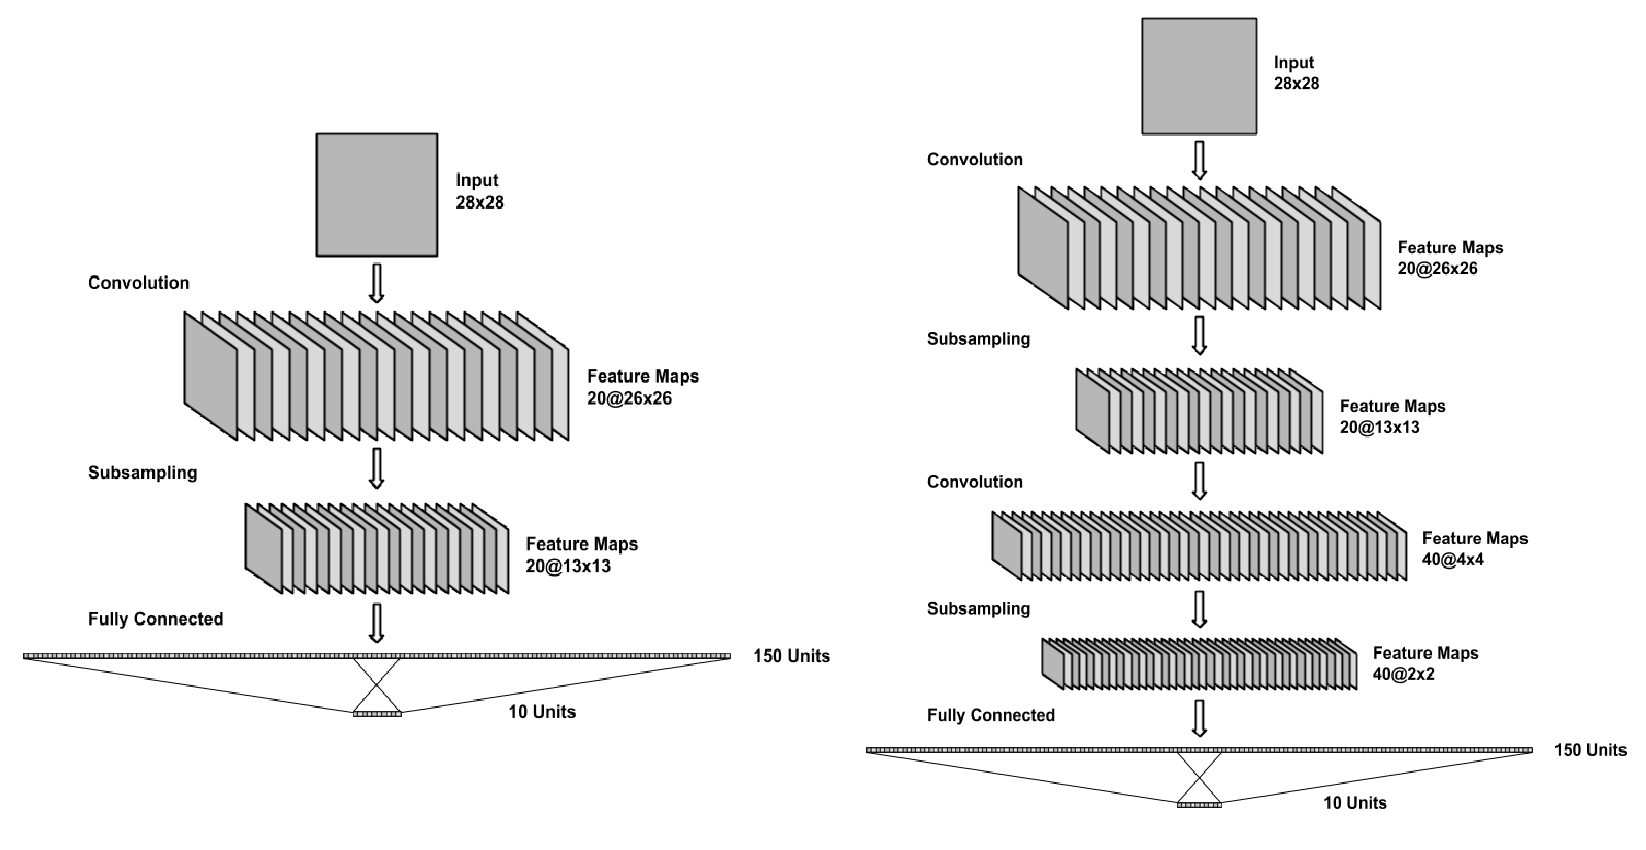
\includegraphics[width=\textwidth,height=8cm]{botharcs}
  \caption{This is a tiger.}
  \label{fig:convarcs}
\end{figure*}

One important suggestion from \cite{EfficientBackProp} that we did not use was the
recommended sigmoid non-linear output function of $f(x) = 1.7159 * tanh(\frac{2}{3}x)$.
While we experimented with the standard sigmoid of $f(x) = \frac{1}{1 + exp(-x)}$,
we used $f(x) = tanh(x)$ for most of our results.

%-------------------------------------------------------------------------
\section{Experiments}

In the following we present the results of the experiments we performed. The experiments were conducted
on one of two architectures. The first architecture was composed of a single convolutional and pooling
layer followed by two fully connected layers. The convolutional layer used 20 filters of size 3x3,
while the max-pooling layer used non-overlapping windows of size 2x2. The first fully connected layer
was composed of 150 units, and the final output layer had 10 units (one per label). The second
architecture added a second set of convolutional and pooling layers before the fully connected layers.
This added convolutional layer had 800 filters of size 8x8, while the added max-pooling layer also used
on-overlapping window size of 2x2. The nonlinearity activation function across both architectures and
all layers was the hyperbolic tangent. A representation of these architectures can be seen in Figure
\ref{fig:convarcs}.

%-------------------------------------------------------------------------
\subsection{MNIST Dataset}

The following experiments were conducted using the MNIST dataset \cite{MNIST}, which includes a training set of
60000 28x28 handwritten digit images and a test set of 10,000 28x28 handwritten digit images.
It is important to note that both the training and test sets are composed of two sets of digits:
an easier set written by US Census Bureau employees and a harder set written by high school students.

%-------------------------------------------------------------------------
\subsection{One Convolutional Layer Architecture}

\subsubsection{Training Set of 500 Images}

The one convolutional/pooling layer architecture was trained for 50 iterations with 50 images per digit
(training set of 500 images), and was subsequently tested on
1,000 new images per digit (test set of 10,000 images).
The training images were taken from the easier portion of the training set, while the test images were taken from
both sets. The results of this training can be seen in Figure \ref{fig:accplot}. The test accuracy was recorded every five training
iterations. An example classification of an image along with the internal state of the trained network is depicted
in Figure \ref{fig:actfilts}. Figure [?] shows examples of correctly and incorrectly classified images.

\subsubsection{Training Set of 1000 Images}

The second experiment with the one convolutional/pooling layer architecture was also trained
for 50 iterations but with 100 images per digit instead of 50 (training set of 1,000 images).
This trained network was then tested on 1,000 new images per digit (test set of 10,000 images).
The results of this training can be seen in Figure \ref{fig:accplot}.
The test accuracy was recorded every five training iterations.
Figure [?] shows examples of correctly and incorrectly classified images.

%-------------------------------------------------------------------------
\subsection{Two Convolutional Layers Architecture}

\subsubsection{Training Set of 500 Images}

The two convolutional/pooling layer architecture was also trained for 50 iterations with 50 images per digit
(training set of 500 images), and was subsequently tested on 1,000 new images per digit
(test set of 10,000 images).
The training images were taken from the easier portion of the training set,
while the test images were taken from both sets.
The results of this training can be seen in Figure \ref{fig:accplot}.
Again, the test accuracy was recorded every five training iterations.
An example classification of an image along with the internal state of the trained network is depicted in
Figure \ref{fig:actfilts}.
Figure [?] shows examples of correctly and incorrectly classified images.

\begin{figure}
  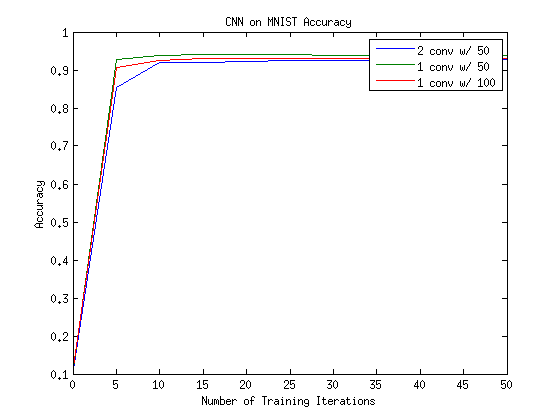
\includegraphics[scale=0.55]{AccPlot}
  \caption{This is also a tiger.}
  \label{fig:accplot}
\end{figure}

\begin{figure*}
  \makebox[\textwidth][c]{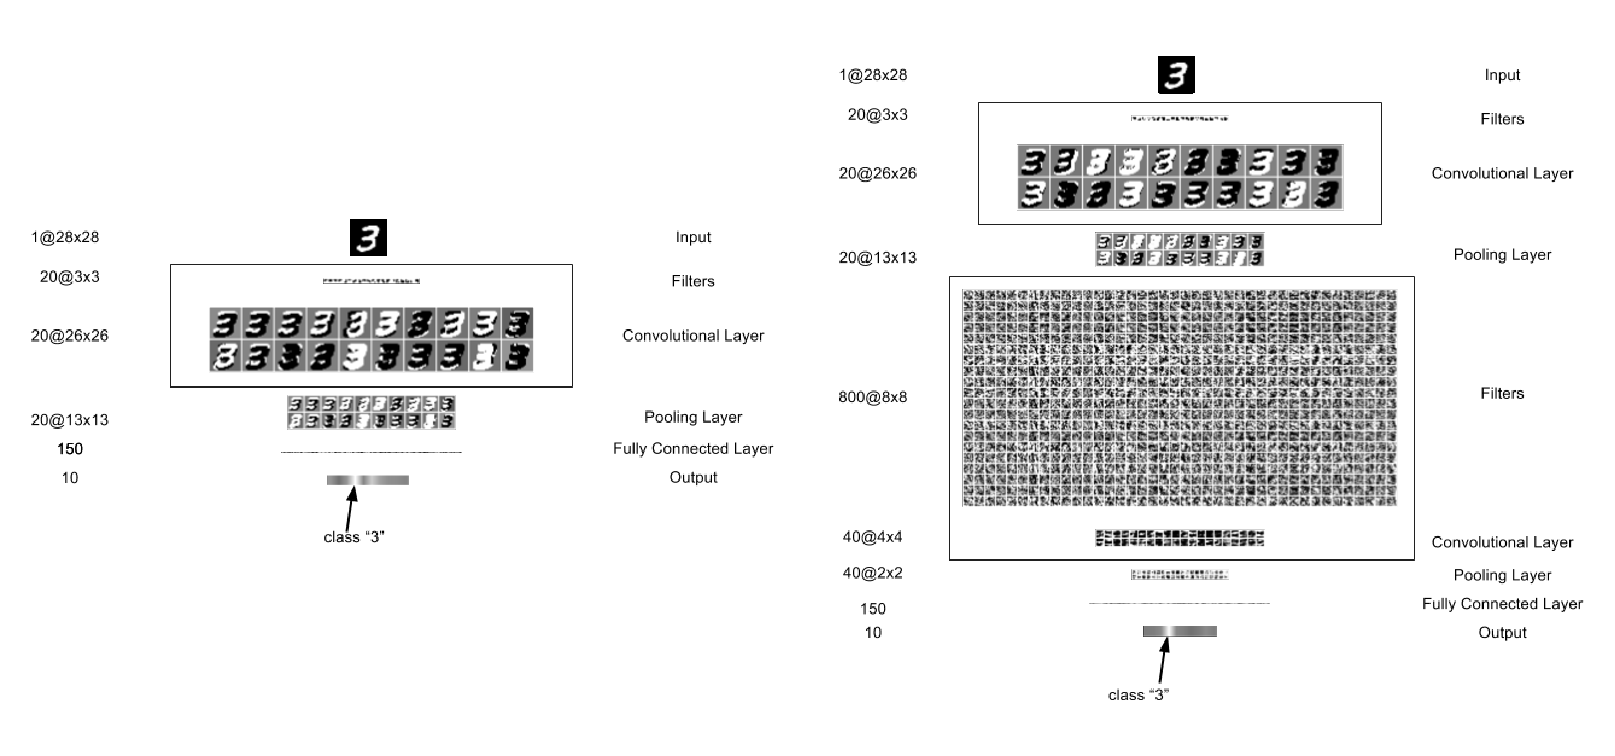
\includegraphics[scale=0.72]{actfilts}}
  \caption{This is also a tiger.}
  \label{fig:actfilts}
\end{figure*}

{\small
\bibliographystyle{ieee}
\bibliography{bib}
}

\end{document}
